
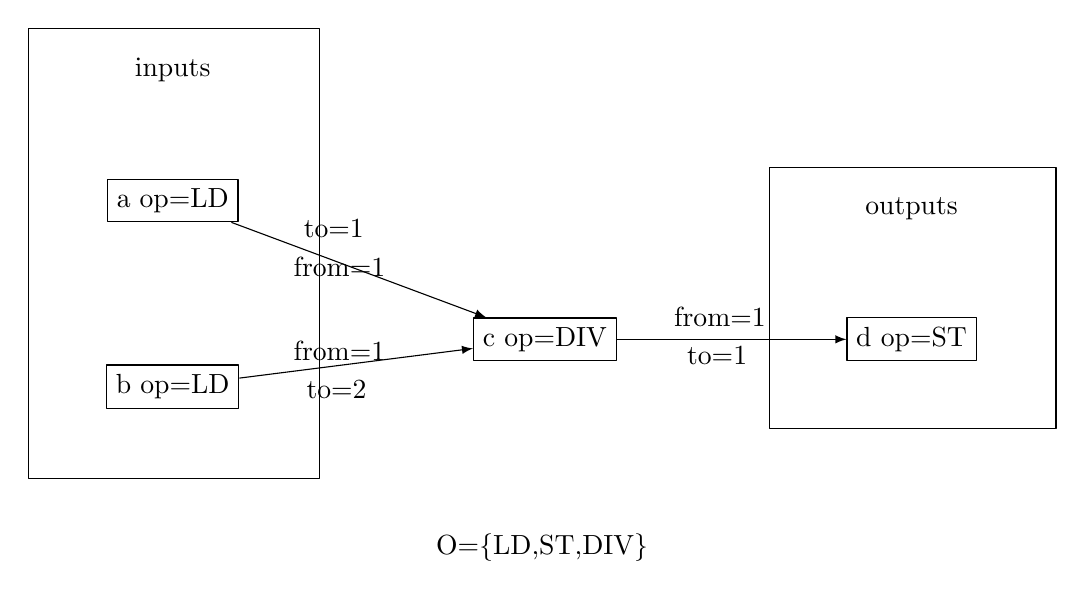
\begin{tikzpicture}[>=latex,line join=bevel,]
%%
\begin{scope}
  \definecolor{strokecol}{rgb}{0,0,0};
  \pgfsetstrokecolor{strokecol}
  \draw (195bp,13bp) node {O=\{LD,ST,DIV\}};
\end{scope}
\begin{scope}
  \pgfsetstrokecolor{black}
  \definecolor{strokecol}{rgb}{0,0,0};
  \pgfsetstrokecolor{strokecol}
  \draw (10bp,38bp) -- (10bp,200bp) -- (115bp,200bp) -- (115bp,38bp) -- cycle;
  \draw (62bp,185bp) node {inputs};
\end{scope}
\begin{scope}
  \pgfsetstrokecolor{black}
  \definecolor{strokecol}{rgb}{0,0,0};
  \pgfsetstrokecolor{strokecol}
  \draw (277bp,56bp) -- (277bp,150bp) -- (380bp,150bp) -- (380bp,56bp) -- cycle;
  \draw (328bp,135bp) node {outputs};
\end{scope}
  \node (a) at (62bp,138bp) [draw,rectangle] {a op=LD};
  \node (c) at (196bp,88bp) [draw,rectangle] {c op=DIV};
  \node (b) at (62bp,71bp) [draw,rectangle] {b op=LD};
  \node (d) at (328bp,88bp) [draw,rectangle] {d op=ST};
  \draw [->] (b) -- (c);
  \draw (121bp,70bp) node {to=2};
  \draw (122bp,84bp) node {from=1};
  \draw [->] (c) -- (d);
  \draw (258bp,82bp) node {to=1};
  \draw (259bp,96bp) node {from=1};
  \draw [->] (a) -- (c);
  \draw (120bp,128bp) node {to=1};
  \draw (122bp,114bp) node {from=1};
%
\end{tikzpicture}

